\documentclass[../main.tex]{subfiles}
\graphicspath{{\subfix{../images/}}}

\begin{document}

\section{Materials and Methods}

\subsection{Equipment}
This research has been conducted on a first-generation \davinci surgical system decommissioned in 2016 and equipped with the dVRK (\davinci Research Kit) framework. The dVRK \cite{Kazanzides2014} is an open-source mechatronics system, consisting of electronics, firmware, and software, that is being used to control research systems based on the first-generation \davinci systems. Based on a ROS \cite{Quigley2009} framework, the dVRK implements high-level accessibility to the sensors, actuators and control algorithms of the \davinci robot, making it more easily interfaceable with advanced strategies and algorithms developed in the most diverse software environments.

The simulator developed for this project renders necessary only the surgeon console, as the ROS messages are sent solely to the virtual surgical scene and not to the physical robot. However, all features of the \psms and of the \ecm are implemented: the \hrsv shows the 3D virtual surgical scene, the \mtms correctly controls the virtual surgical tools, and the clutch foot-switch allows proper repositioning maneuvers. 

\subsection{The Surgical Simulator} 
The objective of investigating a high-specificity aspect regarding the impact of \vfs introduced the necessity of developing an \textit{ad-hoc} surgical simulator with specialized surgical tasks and training exercises: this would allow quantifying surgical performance and monitor training over the key surgical skills as indicated by Smith \textit{et al.} in \cite{Smith2014}. 

The simulator is based on \textit{Unity}, a cross-platform game engine that allows the development of 3D applications and games. The Unity engine is a powerful tool for the development of virtual environments, as it allows the creation of complex 3D scenes with a high level of realism, and the implementation of complex interactions between the virtual objects and the user. Specifically, the simulator implements gravity, object collisions and manipulation. A 3D model of the \davinci patient cart is present in the simulator and responds in real-time to the ROS messages received from the console, therefore the virtual \psms replicate the motion of the real ones. 

Two virtual cameras are positioned in the Unity scene on the tip of the endoscope mounted on the \ecm: the horizontal distance between the two virtual cameras ($5.3 \unit{mm}$) matches the one of the real endoscope, as does the Field-of-View ($80 \unit{deg^2}$). The feeds of the virtual cameras, rendering the 3D scene in real-time, are sent separately to the two oculars of the \hrsv. The slightly different images from the left and right eye yield the sensation of depth perception and allow the user to perceive the virtual scene in three dimensions, as it happens when teleoperating with the real robot. 

The training surgeon interacts with the console in the same exact way as he would when teleoperating the real robot: he views the surgical scene in the oculars, the virtual instruments respond in real-time to the movements of the manipulators and with the same kinematics, and the 3D objects behave in the same way as they would if they were real thanks to the simulated physics computed by the Unity Engine.   

\subsubsection{The Surgical Tasks}
The simulator comprises eight surgical tasks, four of which (\textit{Path, Rings, Pillars} and \textit{Exchange}) are simplistic training tasks built with objects of simple geometry, while the remaining four (\textit{Liver Resection, Nephrectomy, Thymectomy} and \textit{Suturing}) emulate \textit{in-vivo} surgical procedures and are therefore more realistic. Fig.\ref{fig:taskspanel} collects snapshots of the tasks. All of these are constructed and set up in order to be as challenging as possible in relation to a specific surgical skill. Specifically:

\begin{itemize}
  \item \textit{Path} and \textit{Liver Resection} require articulate wrist motion and stability
  \item \textit{Rings} and \textit{Nephrectomy} survey the depth perception skills
  \item \textit{Pillars} and \textit{Thymectomy} are hand-eye coordination tasks
  \item \textit{Exchange} and \textit{Suturing}, both bi-manual tasks, challenge the capabilities in terms of instrument exchange 
\end{itemize}

\begin{figure}
    \centering
    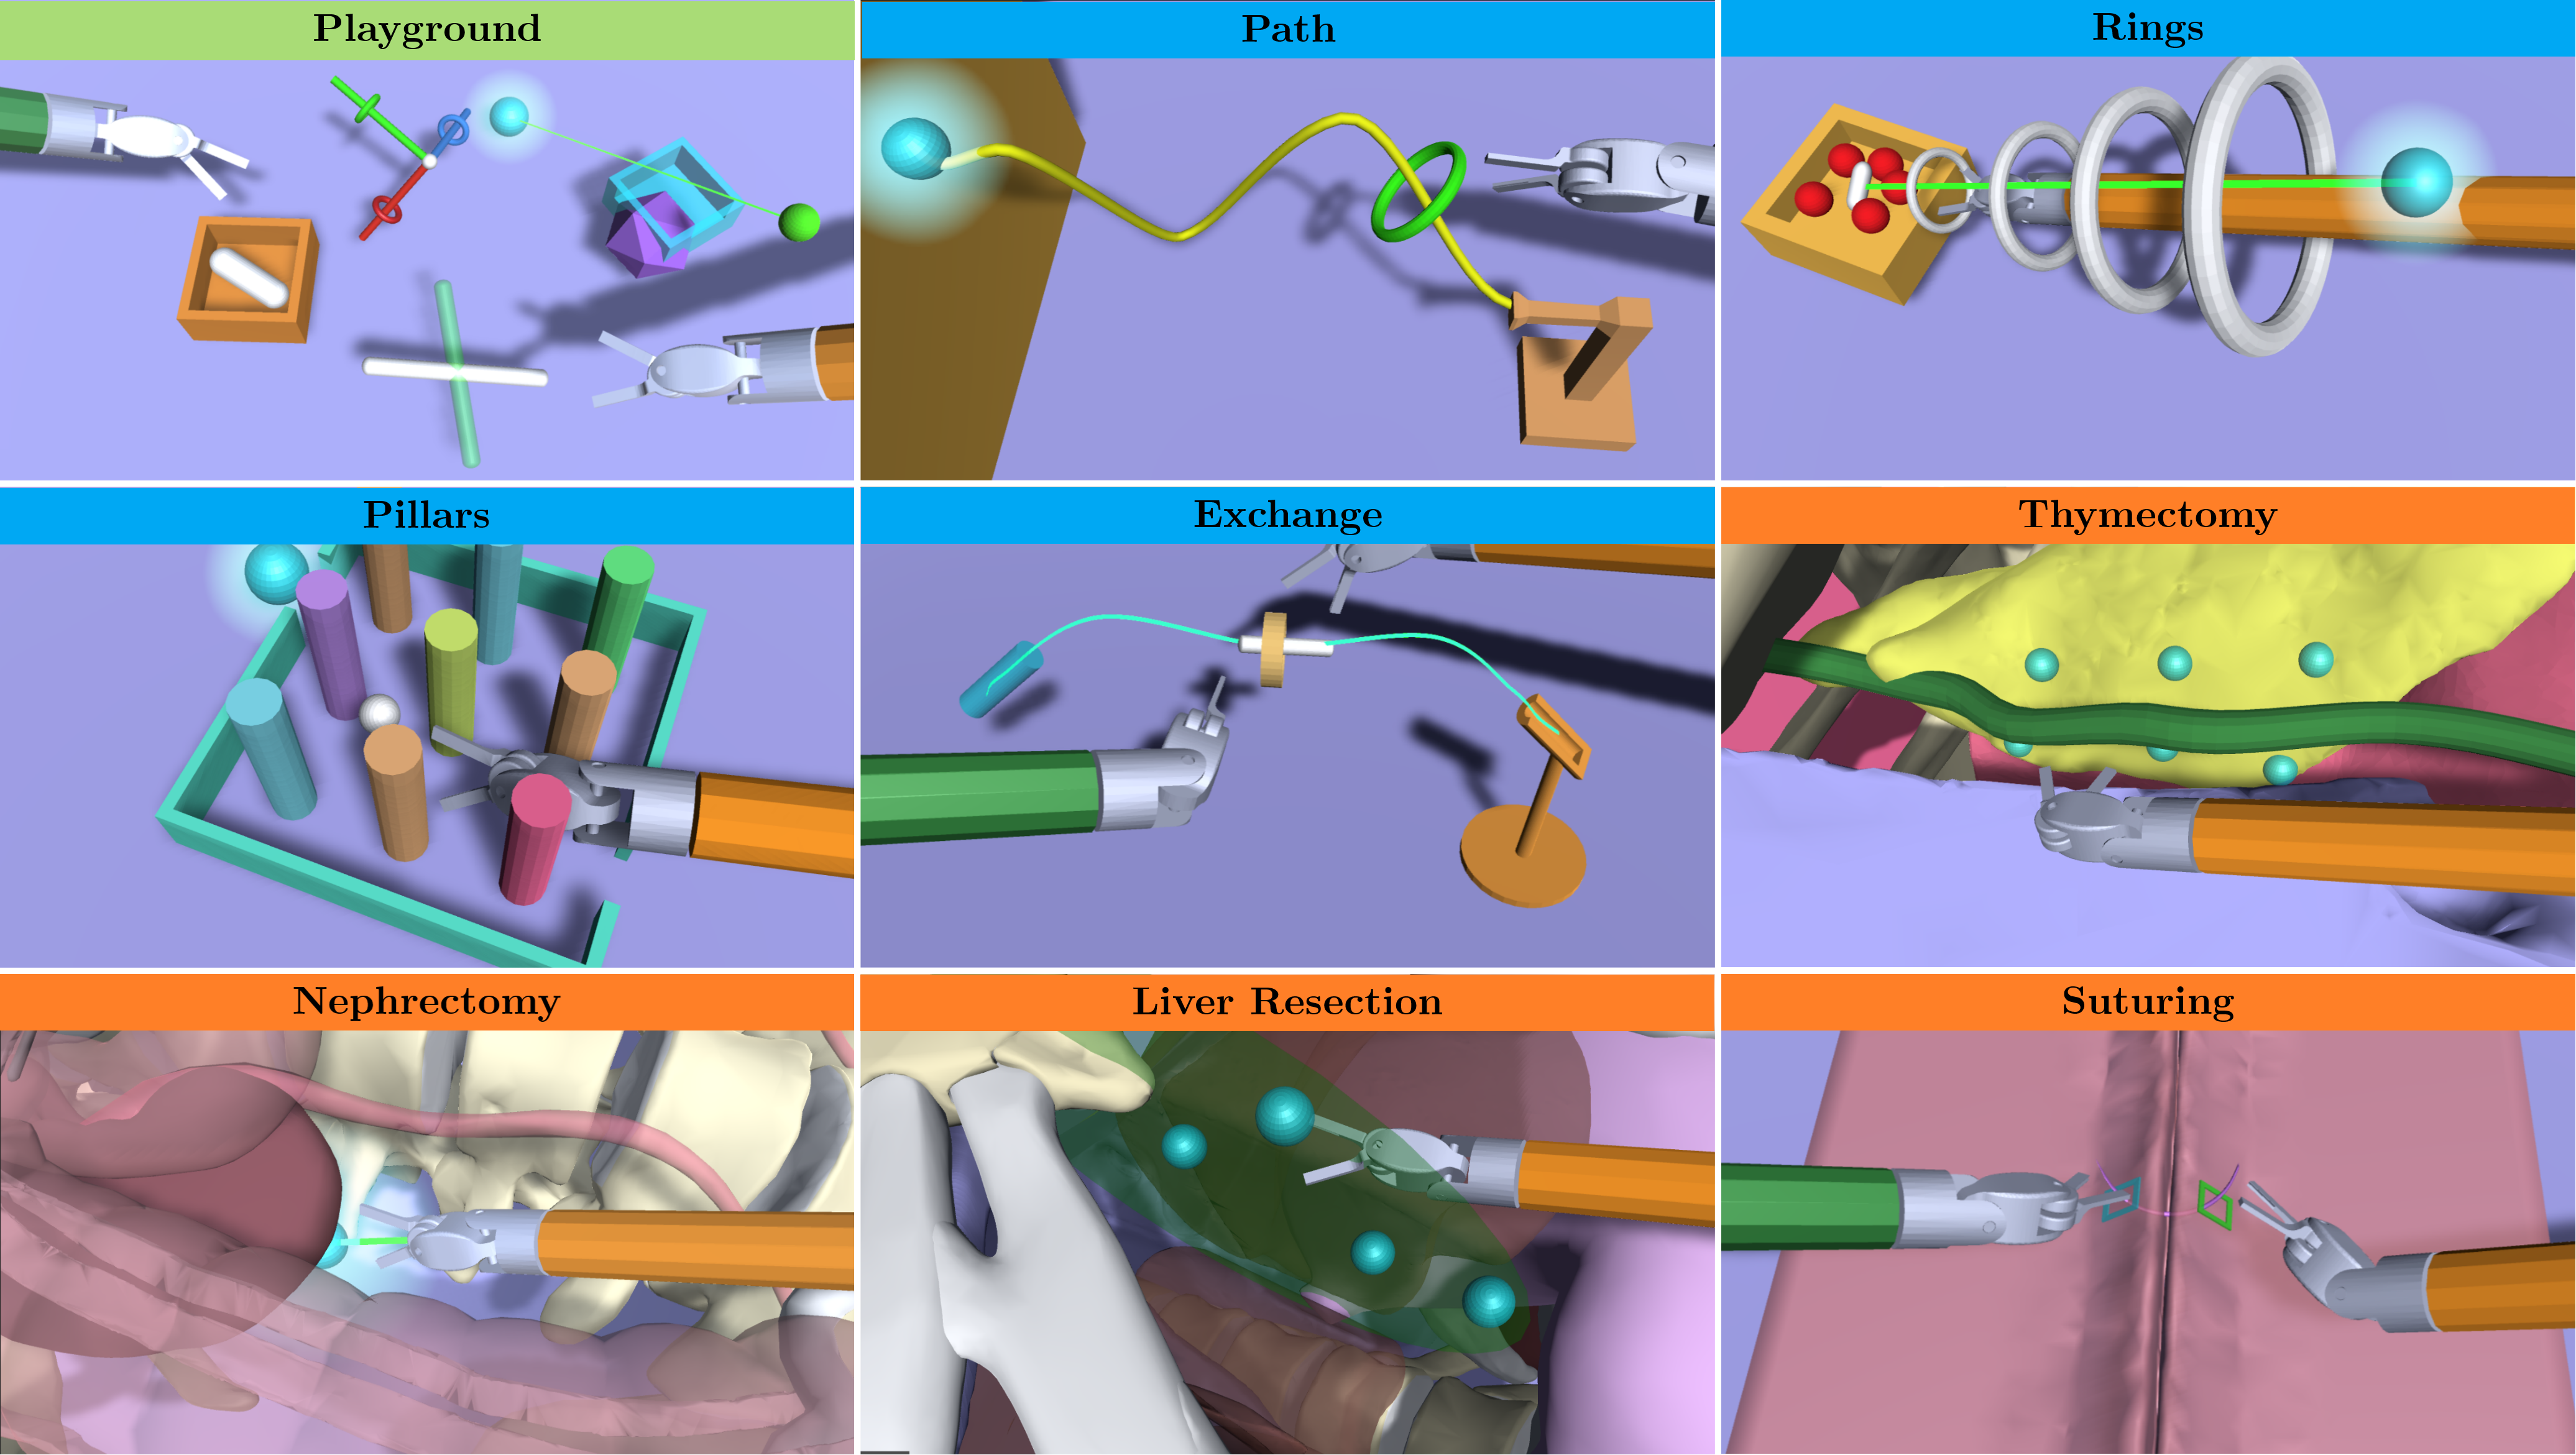
\includegraphics[width=\textwidth]{images/tasks_panel.png}
    \caption{Snapshot of the simulated surgical tasks, with the respective denomination. Training tasks have blue headlines, while realistic evaluation tasks have orange headlines. \textit{Playground} is a propaedeutic task and isn't featured in the experimental study}
    \label{fig:taskspanel}
\end{figure}

\paragraph{Path} Objective of this task is to grab a torus-like object and carry it along a reference trajectory. To achieve this, discrete wrist articulation and motion smoothness are required. The reference trajectory is set up in order to require a wrist rotation of at least $90 \unit{deg}$ around 2 perpendicular axes, the one pointing from right to left and the one pointing forward with respect to the camera view.
\paragraph{Rings} In this task, the operator is required to precisely insert the instrument inside a narrow constrained space defined by a set of increasingly smaller rings, grab a target object and carry it out of the constrained space. The task tests the depth perception skills of the operator, as the rings are positioned at an angle with respect to the camera view.
\paragraph{Pillars}
\paragraph{Exchange}
\paragraph{Thymectomy}
\paragraph{Nephrectomy}
\paragraph{Liver Resection}
\paragraph{Suturing}
\paragraph{Playgrounf}

\subsection{Virtual Fixtures}
\subsection{Clinical Validation}
\subsection{Experimental Protocol}
\subsection{Performance Metrics}


% BIBLIOGRAPHY
\bibliographystyle{unsrt}
\bibliography{refs.bib}

\end{document}